\begin{frame}{The Multi-agent simulation}
\begin{block}{Simulation model}
\begin{columns}
\begin{column}{.18\linewidth}
    \begin{figure}
	
\includegraphics[width=.4\textwidth]{figures/electric-car.png}
	
\includegraphics[width=.4\textwidth]{figures/charging.png}
    \end{figure}
\end{column}
\begin{column}{.78\linewidth}
\begin{itemize}
    \item Ex: SkuadCityModel, SmartCityModel
    \item Schematic representation of reality in order to study and to understand it
    \item Composed of a set of autonomous entities (agents) located in environments and interacting according to relationships
    \item \alert{Space} and \alert{organization} are modeled as \alert{environments} : allows the exchange of spatial and social information
    \item Agent behavioural cycle: perception, decision, action/influence 
\end{itemize}
\end{column}
\end{columns}
\end{block}
\begin{block}{Simulation platform}
\end{block}


\note{
Une simulation multi-agents peut se diviser en deux grandes parties: la plateforme de simulation et le modèle de simulation. Le modèle de simulation propose une représentation schématique de la réalité en vue de l’étudier et de la comprendre. Il est composé des agents, des environnements ainsi que des relations qui les permettent d'interagir. Dans la plupart des modèles, l’environnement est soit un environnement spatial, soit un environnement de communication dont un cas particulier est l’environnement social. Ces environnements permettent aux agent d'échanger des données relatives aux contextes d’activation spatiales et sociales. La relation entre l’agent et son environnement se traduit par le fait que l’agent agit ou exerce une influence sur son environnement et le perçoit.  Le cycle comportemental classique d’un agent se résume alors en trois phases: une phase de perception où il récolte des informations contenues au niveau de l’environnement, une phase de délibération où l’agent active son processus de raisonnement et choisi un comportement à exécuter en fonction des percepts qu’il aura récolté et de son état interne et une phase d'action ou d’influence où l’agent agit ou essaie d’agir sur son environnement.
}
\end{frame}

\begin{frame}{The Multi-agent simulation}
\begin{block}{Simulation model}
\end{block}
\begin{block}{Simulation platform}
\begin{columns}
\begin{column}{.18\linewidth}
    \begin{figure}
	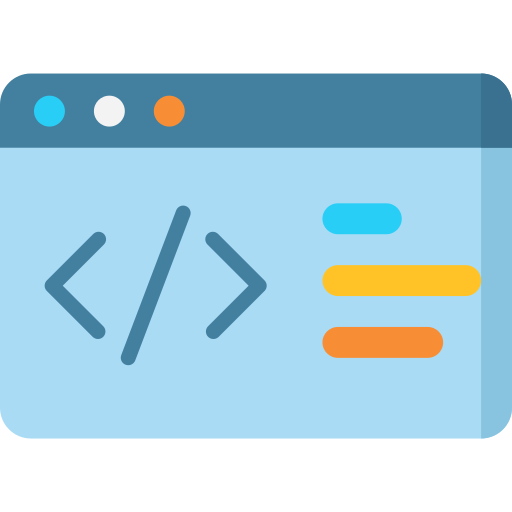
\includegraphics[width=.4\textwidth]{figures/code.png}
	
\includegraphics[width=.4\textwidth]{figures/calendar.png}
    \end{figure}
\end{column}
\begin{column}{.78\linewidth}
\begin{itemize}
    \item Ex : SimSKUAD, Repast Simphony
    \item Dedicated to multi-agent simulation development
    \item Contain libraries that facilitates the development of multi-agent simulation. Ex: the scheduler
\end{itemize}
\end{column}
\end{columns}
\end{block}


\note{
La plateforme de simulation multi-agents est dédiée au développement de systèmes et simulations multi-agent. Elle peut contenir un ensemble de librairies facilitant le développement d'un modèle de simulation. Plus particulièrement, puisque nous nous intéressons au temps, les plateformes de simulation comme celles que nous utilisons dans le cadre de cette thèse contiennent l'ordonnanceur de la simulation. }
    
\end{frame}

\begin{frame}{The Time management in multi-agent simulation}
\begin{block}{The Scheduler}
\begin{itemize}
        \item Is responsible for the simulation activation cycle
        \item Consists of a mechanism that makes time run out, activates the agents and updates the environments according to a virtual clock (\textbf{simulated time} $\ne$ real time)
        \item Uses time scheduling approaches. Ex : time-stepped, event-driven, hybrid, temporality model
    \end{itemize}
\vspace{.5cm}
\textbf{Main limit}: No access to (no exchange of) information about the agents temporal activation dynamic
\end{block}
    
    \note{
    
    Cet ordonnanceur est responsable de la gestion du temps en terme de cycle d’activation de la simulation. Son fonctionnement consiste en une mécanique qui fait écouler le temps, qui active les agents et met à jour les environnements en fonction d’une horloge virtuelle. Nous parlons notamment de temps simulé qui est le reflet de notre temps réel, astronomique. C'est le temps qui est mesuré par une horloge virtuelle intégrée dans le simulateur. Pour gérer ce temps simulé, l’ordonnanceur utilise différentes approches d’ordonnancement : à pas de temps constant, événementielle, hybride, etc. La manière dont le temps est géré est différent selon l’approche utilisé, ainsi chaque approche peut avoir ses avantages et ses limites. Cependant celle que nous retiendrons est le fait qu'aucune approche ne permet aux agents, l'accès aux informations sur leurs dynamique d'activation temporelle.
    
    }
\end{frame}

\begin{frame}{The Time management in multi-agent simulation}
%flèche dans les deux sens ambigüe
\begin{columns}
\begin{column}{.18\linewidth}
    \begin{figure}
	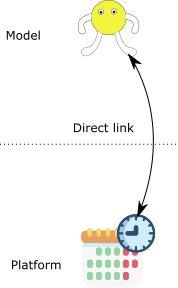
\includegraphics[width=1.2\textwidth]{figures/agentsVSscheduler.png}
    \end{figure}
\end{column}
\begin{column}{.78\linewidth}
\textbf{Process}:
\begin{itemize}
    \item The agent or the simulation model determines the activation rythm and communicates it to the scheduler
    \item The scheduler activates the agents based on this information.
\end{itemize}
    \vspace{1cm}
\par \textbf{Main limit}: no exchange of information about the agents temporal activation dynamics
        \begin{itemize}
            \item  Sharing temporal activation dynamics information is possible
            \item Access to temporal activation dynamics information is not possible (a key smart cities effectiveness)
            \item Taking into into account \say{non-existent} information in the agents reasoning is not possible
        \end{itemize}

\end{column}
\end{columns}
    
\note{
De manière générale, la relation entre l’agent et l’ordonnanceur se fait par lien direct. En fonction de l'approche d'ordonnancement utilisé, l'agent ou le modèle de simulation détermine le rythme d’activation et le communique à l'ordonnanceur de la simulation, au niveau de la plateforme de simulation. L’ordonnanceur active donc les agents en fonction de ces informations. Le traitement de l’information se fait dans un seul sens : aucun échange d’informations ne peut être effectué au niveau de la dimension temporelle: l'agent partage des informations sur sa dynamique temporlle mais n'a pas accès à ces informations partagées donc impossible de les prendre en compte au niveau du raisonnement. Voyons plus en détails comment nos propositions permettent de nous affranchir de ces limites.


}
\end{frame}